% !TEX root = ../main.tex
\section{System Overview}

\begin{figure}[htbp]
    \centering
    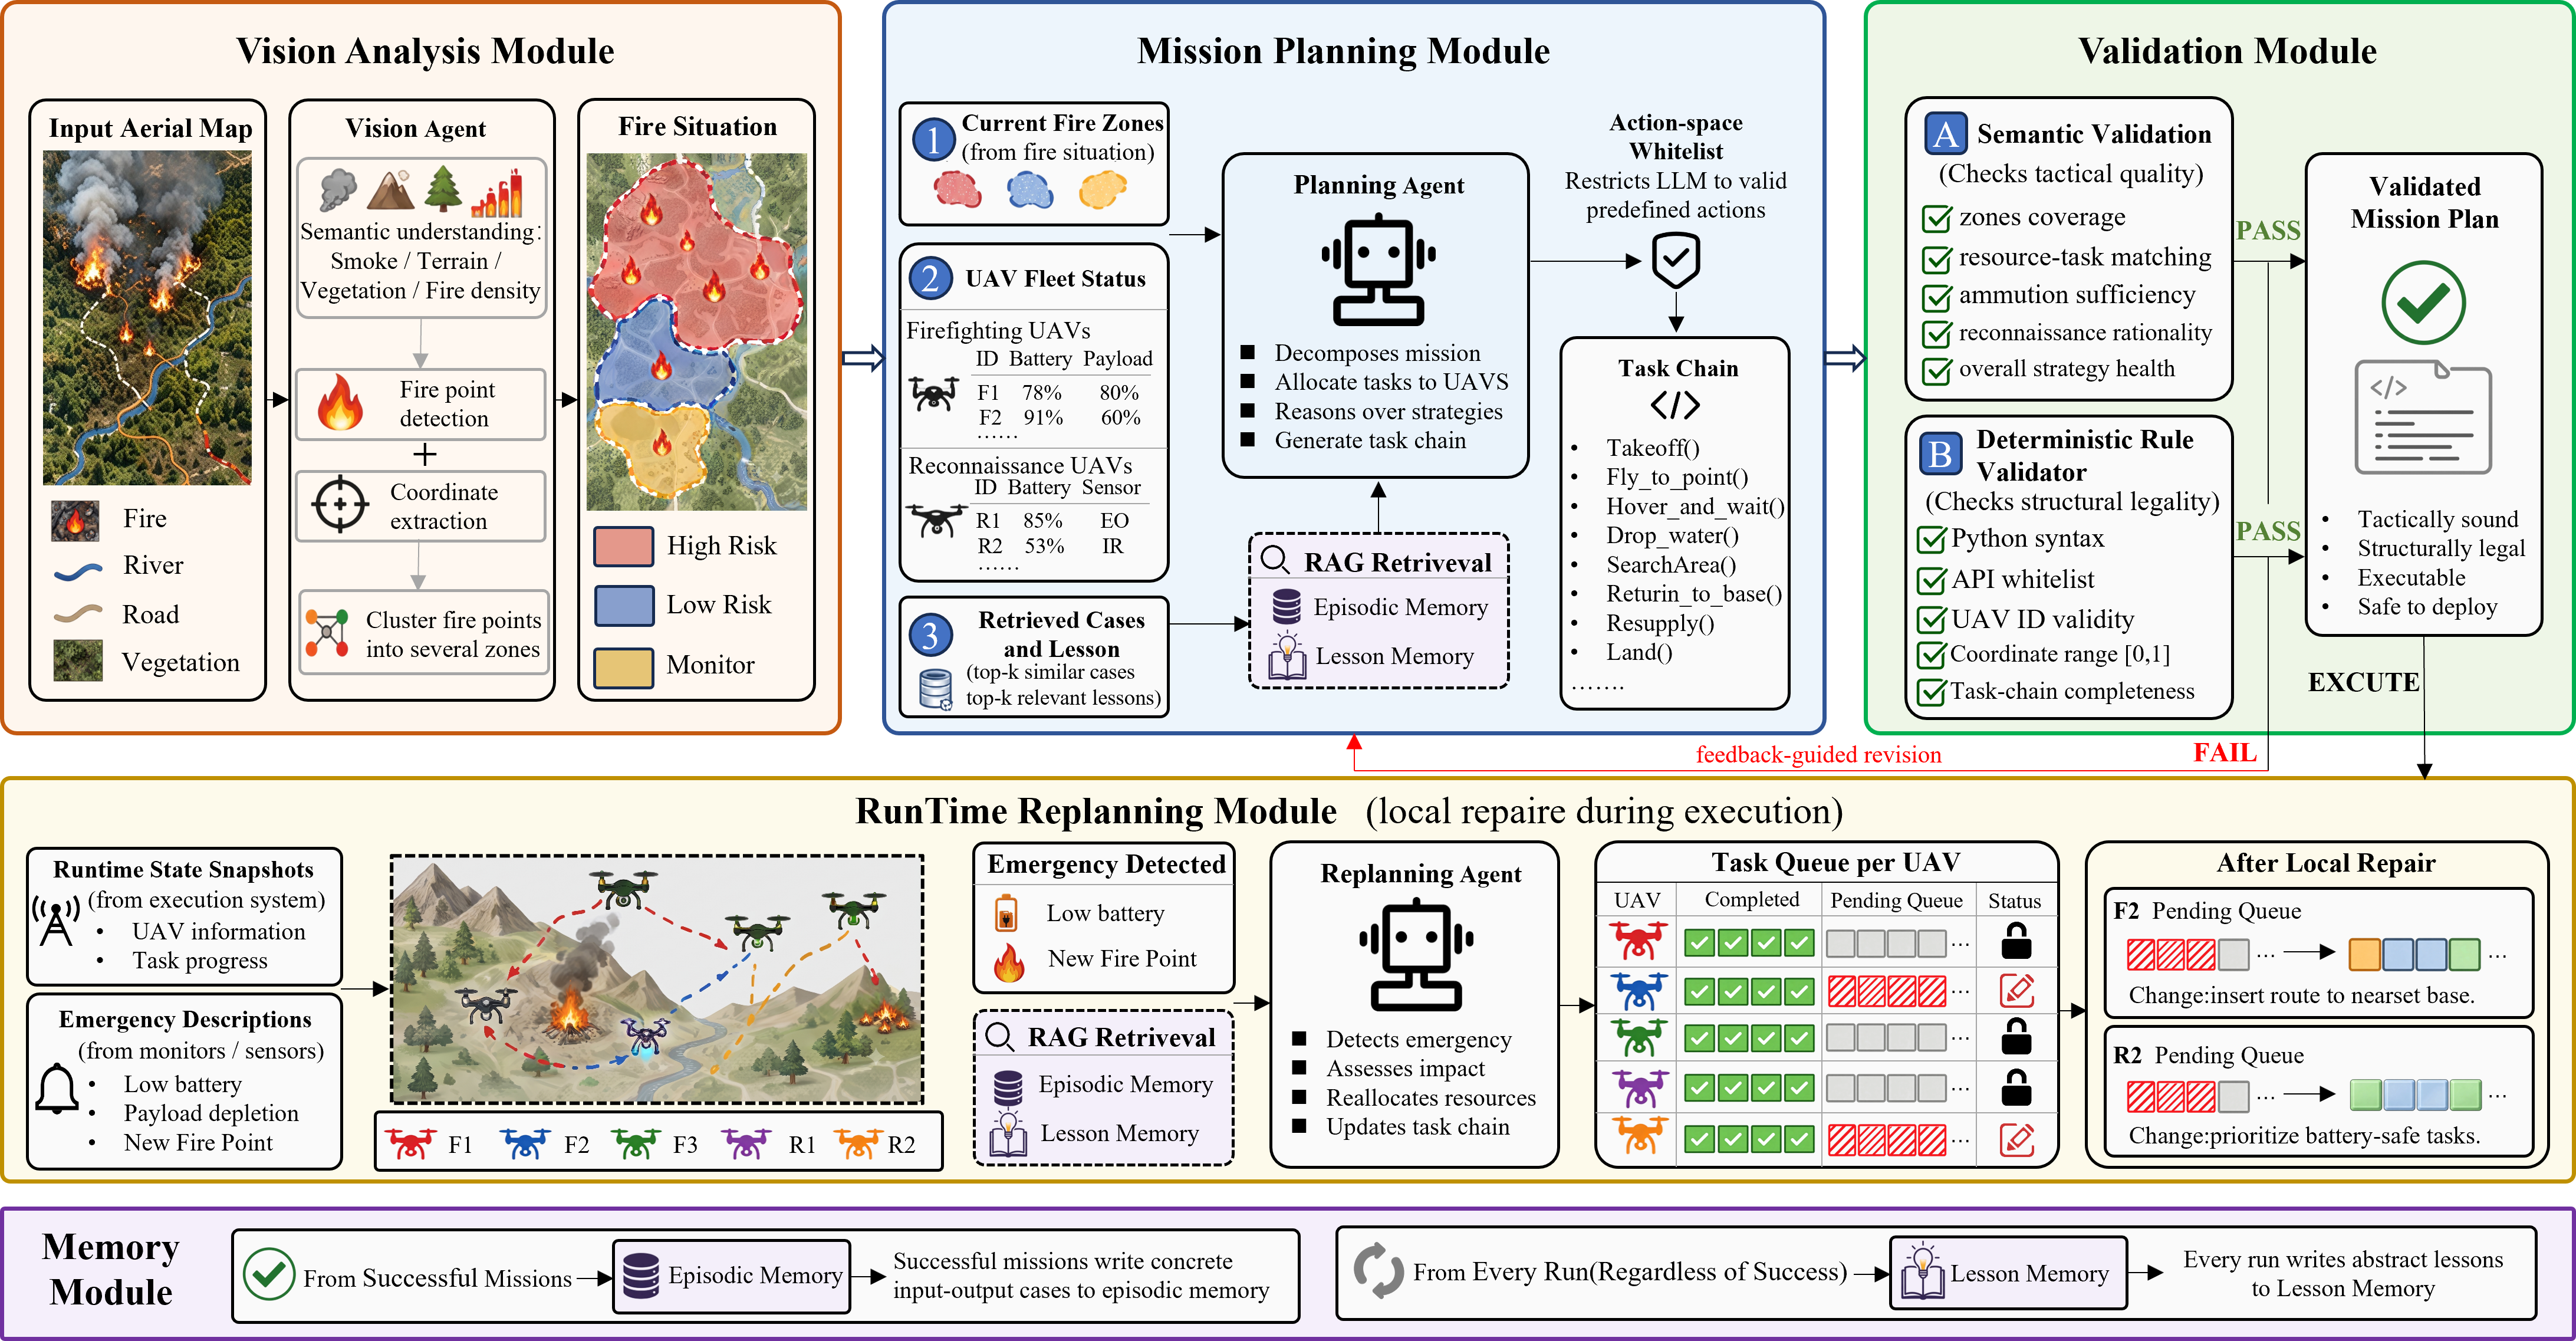
\includegraphics[width=1\textwidth]{figures/system}
    \caption{Overview of the proposed system.}
    \label{fig:method-overview}
\end{figure}

Central to the proposed system is the separation between initial mission generation,
independent plan checking, runtime adaptation, and experience reuse.
The system takes aerial fire imagery as the initial input and produces
an executable mission plan for a multi-UAV fleet.
The main planning pipeline contains three modules:
Vision Analysis, Mission Planning, and Validation.
A Runtime Replanning module operates outside the pipeline and adjusts the plan
when unexpected events occur during execution.
Two memory modules, Episodic Memory and Lesson Memory, supply past experience
to the planning and replanning modules.
Figure~\ref{fig:method-overview} shows this overall structure.

\paragraph{Vision Analysis.} Vision Analysis converts raw aerial imagery
into a structured description of the fire situation.
This module uses a multimodal LLM to perform two tasks in a single inference pass.
First, it detects all visible fire points in the image and outputs their normalized coordinates.
Second, it clusters these points by spatial density, partitioning the continuous fire field
into several discrete task zones.

This module uses a multimodal LLM rather than a vision-only model because zone division
depends on more than fire point locations.
The division also depends on visual context, such as smoke, vegetation,
and terrain boundaries.
These cues require joint reasoning over appearance and spatial semantics.

\paragraph{Mission Planning.} Mission Planning is the core decision module.
It converts the structured fire situation produced by Vision Analysis into an executable
multi-UAV collaborative plan. A planning LLM generates a complete task chain for each
UAV in the fleet, covering task allocation, temporal sequencing, and endurance management.
To keep outputs controllable, the LLM is restricted to a predefined set of allowable actions.

Mission Planning combines the fire situation, retrieved experience,
and operational constraints.
It receives the structured fire situation from Vision Analysis,
retrieves relevant past cases and lessons from both memory modules,
and produces a coordinated plan in which each UAV's task chain respects
the fleet's capabilities and the mission's operational constraints.

\begin{figure}[htbp]
    \centering
    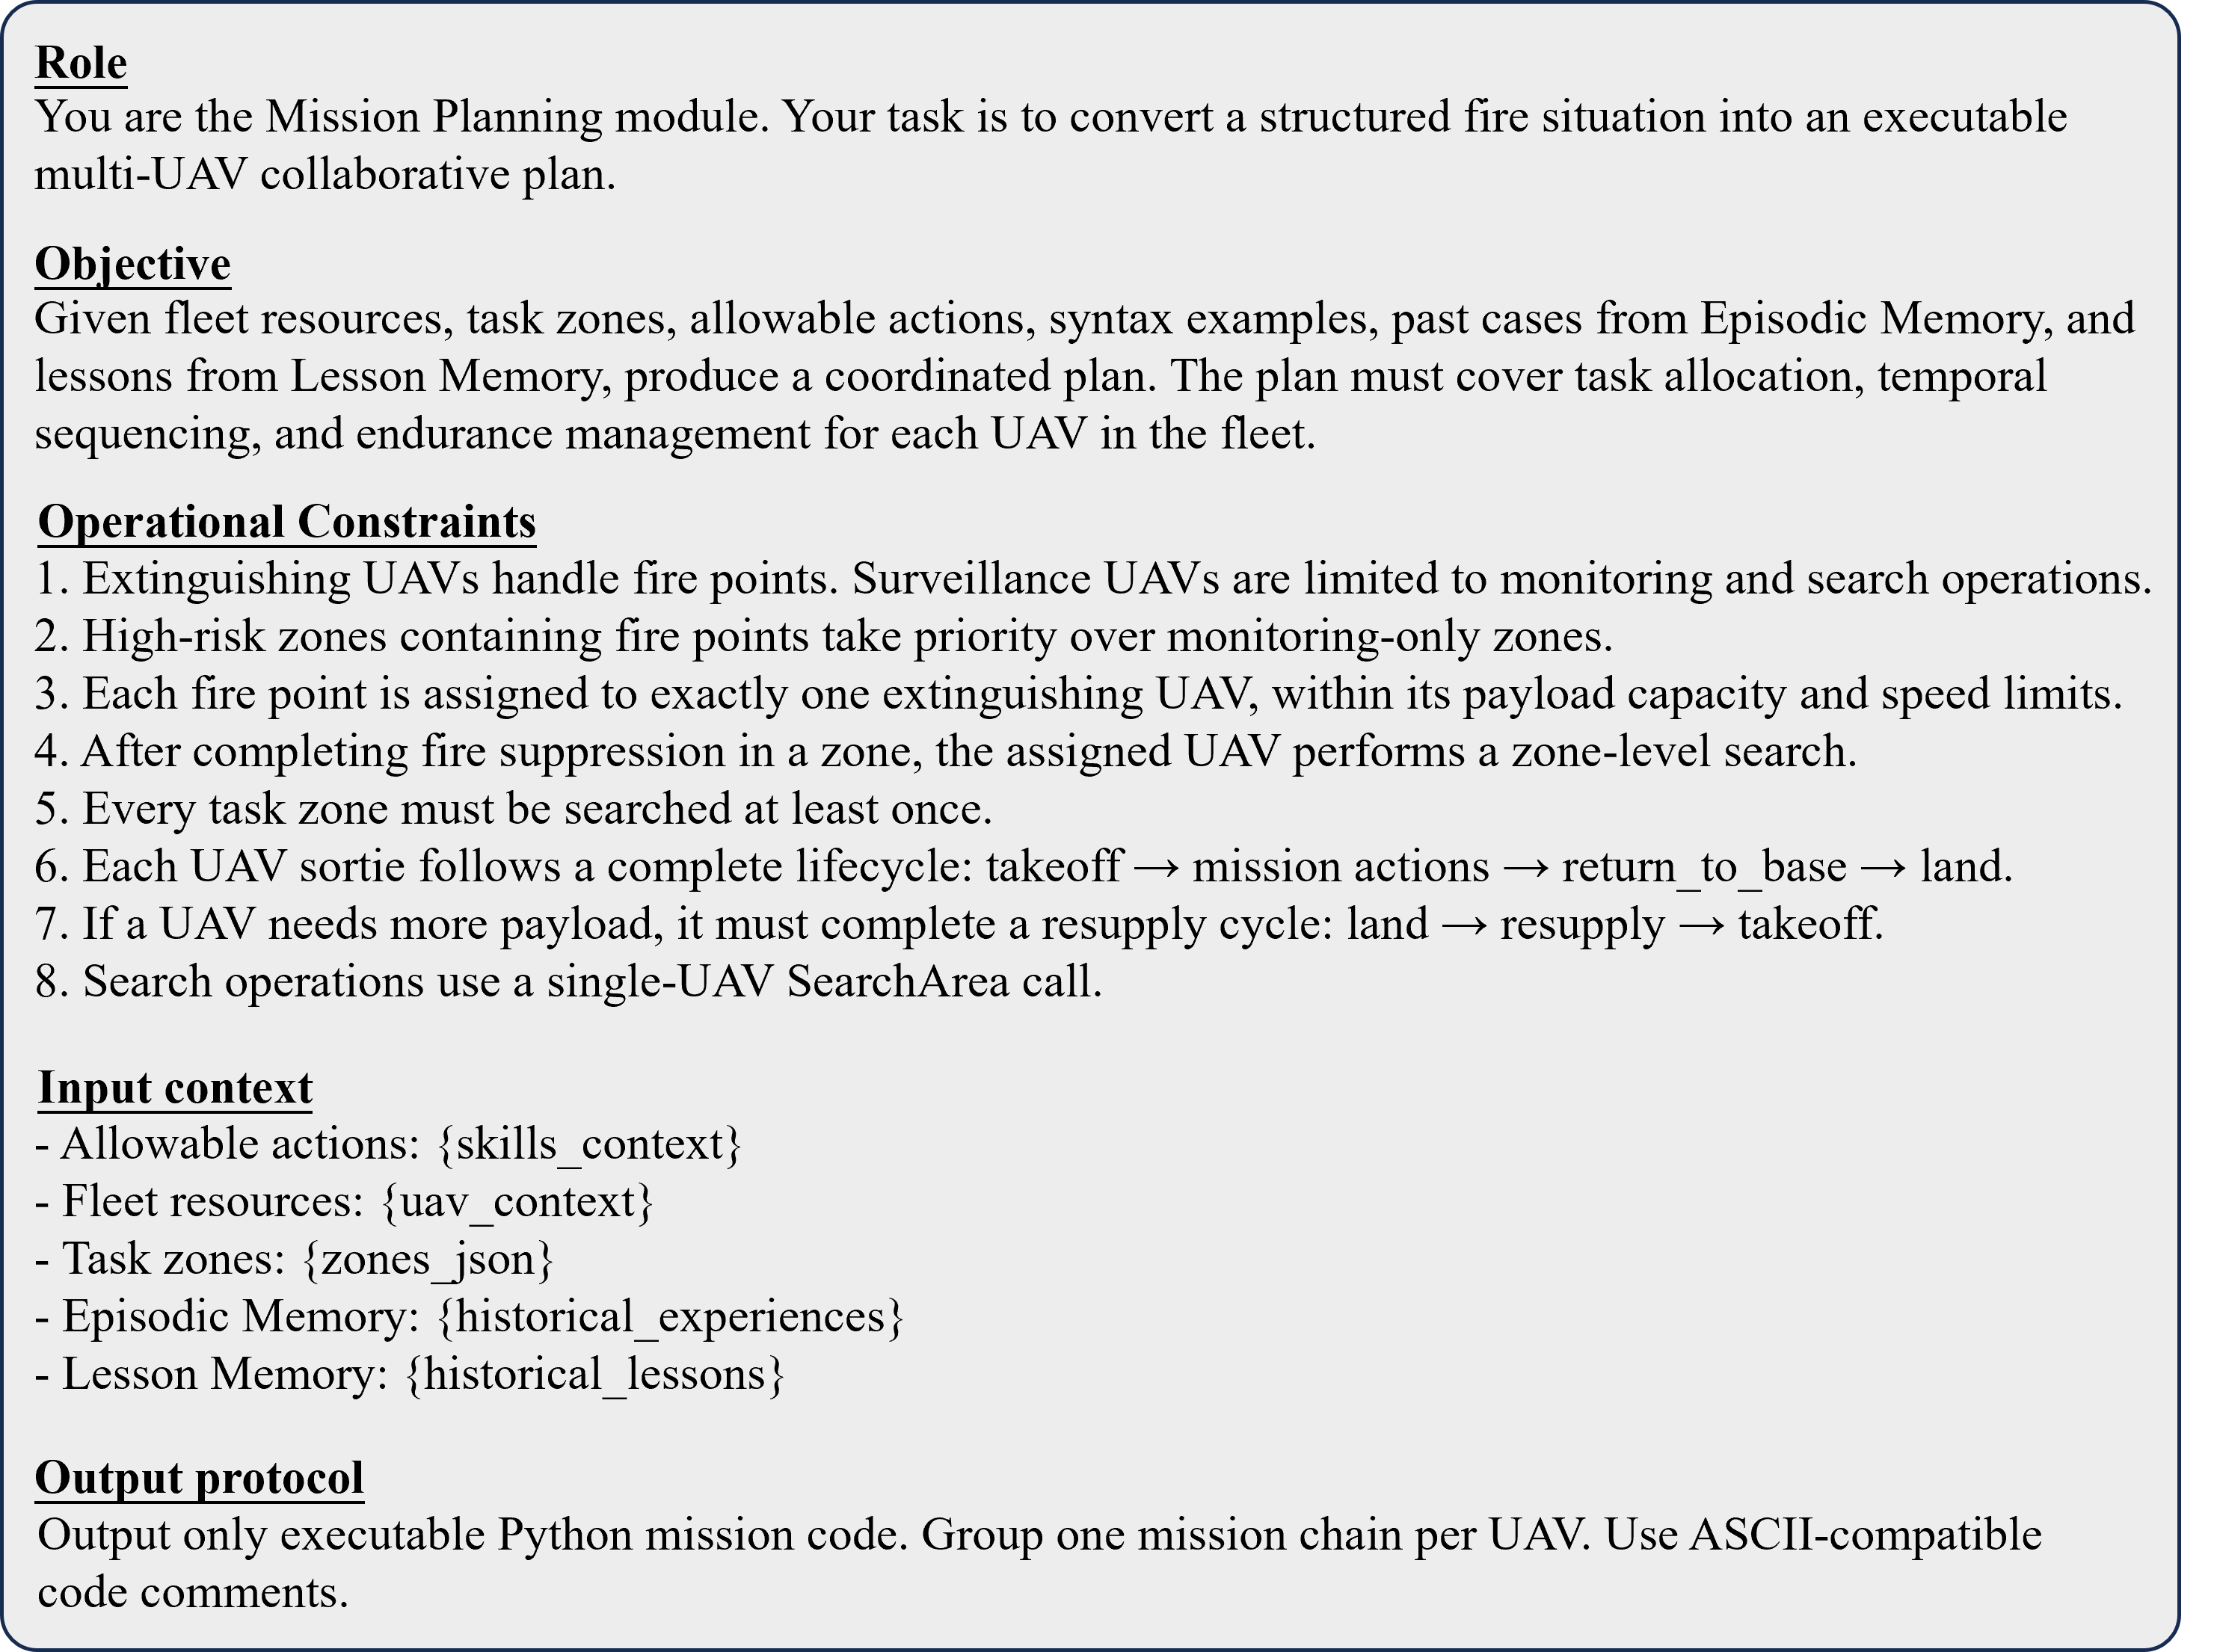
\includegraphics[width=0.8\textwidth]{figures/prompt}
    \caption{The prompt template used by the Mission Planning module.}
    \label{fig:planning-prompt}
\end{figure}

The prompt template for the planning LLM is shown in Figure~\ref{fig:planning-prompt}.

\paragraph{Validation.} The Validation module assesses each candidate plan through
two sequential checks. Together, the two checks form the audit--correction loop:
when either one rejects a plan, its feedback is routed back to Mission Planning for revision.
This loop turns validation failures into targeted feedback for the next planning attempt.

The first check, Semantic Validation, uses an independent LLM to evaluate the plan
from a tactical rationality perspective. It examines zone coverage completeness,
resource-task matching, payload adequacy, and overall strategic health.
Using a separate LLM rather than asking the planning LLM to self-check
avoids self-consistency bias.

The second check, Deterministic Rule Validation, uses a rule engine to verify
structural legality, including UAV existence, coordinate validity, and task chain
completeness. Unlike the semantic check, this rule check asks whether the plan
is structurally legal.
This question can be answered deterministically within the defined rule set.


\paragraph{Runtime Replanning.} This module handles unexpected events during mission execution.
It takes a runtime state snapshot as input, including current positions, battery levels,
payloads, and task progress for each UAV.
Its output is not a new global plan, but a local revision of the current plan.
Unlike the main pipeline, Runtime Replanning reasons about a dynamic execution state and
changes only the affected part of the plan.

When a replanning event occurs, the module retrieves similar fault scenarios
from Episodic Memory as repair references.
These cases describe how comparable failures were resolved in past missions,
providing the replanning LLM with tactical precedents for the current situation.

\paragraph{Memory System.} The Memory System allows the system to reuse past experience.
The two memory modules differ in what they store and how their contents are used.

Episodic Memory stores concrete successful cases as input--output pairs.
Each case records the situation, the generated or revised plan,
and the corresponding outcome.
Cases are indexed by situational features, so that when a new scenario arises,
the system retrieves the most similar past cases as tactical references.

Lesson Memory serves a different role. Instead of storing concrete cases,
it keeps higher-level lessons distilled from every run.
After each mission, an LLM reviews the full execution trace.
The trace includes the initial plan, validation feedback, runtime events,
replanning actions, and final scores.
The LLM then extracts concise, reusable lessons.
These lessons capture patterns such as common planning mistakes, resource estimation biases,
and effective repair strategies.

\section{Benchmark Design}

Building on the proposed closed-loop rescue system, we design a benchmark that
evaluates its perception, planning, and replanning capabilities under
real-UAV-informed conditions.

To evaluate the system described above, we design a benchmark for
UAV-assisted forest fire rescue.
The benchmark targets closed-loop decision-making along a continuous chain:
aerial fire situation analysis,
resource-constrained mission planning, and runtime replanning.
This chain captures the full decision workflow, from raw aerial imagery
to an executable and adaptable multi-UAV plan.
The task is broader than fire detection alone.
It is also broader than task allocation alone.
A model must handle this full decision chain within a single
evaluation instance.

Existing benchmarks only partially cover this full decision chain.
Vision benchmarks cover aerial objects, fire, and smoke.
They usually focus on detection, tracking, classification, or segmentation
\cite{xia2018dota,zhu2022visdrone,mowla2024uavsffdb,shamsoshoara2021flame,han2024msfsdb}.
They stop at visual understanding and do not evaluate downstream rescue decisions.
Some benchmarks move beyond perception.
Wildfire VQA and disaster-oriented multi-agent benchmarks evaluate multimodal reasoning,
task allocation, path planning, or coordinated response
\cite{habibpour2026wildfirevqa,kleiner2013rmasbench}.
However, these capabilities are still tested separately.
They are not coupled into a single rescue loop.
A complete evaluation loop would couple forest fire perception
with disaster semantics, UAV-level constraints and runtime replanning. 
Crisis-response benchmarks mainly focus on text-based situational assessment and 
humanitarian information classification, supporting macro-level awareness 
but not fine-grained UAV task execution \cite{alam2021crisisbench}. 
This creates a mismatch between existing evaluation settings
and the closed-loop rescue process targeted in this work.
Table~\ref{tab:benchmark_comparison} summarizes this comparison
across four capability dimensions.

% Required packages:
% \usepackage{booktabs}
% \usepackage{makecell}
% \usepackage{pifont}
% \usepackage{xcolor}
% \usepackage{graphicx}

\newcommand{\cmark}{\textcolor{green!60!black}{\ding{51}}}
\newcommand{\xmark}{\textcolor{red}{\ding{55}}}
\newcommand{\pmark}{\textcolor{orange!85!black}{\textbullet}}

\begin{table}[!htbp]
\centering
\caption{Coverage of evaluation capabilities in existing datasets, benchmarks,
and the evaluation suite used in this work.
\cmark indicates explicit coverage, \pmark indicates partial coverage, and \xmark indicates no explicit coverage.}
\label{tab:benchmark_comparison}
\resizebox{\textwidth}{!}{
\begin{tabular}{lcccc}
\toprule
\textbf{Benchmark / Dataset}
& \textbf{\makecell{Forest Fire\\Perception}}
& \textbf{\makecell{Disaster\\Semantics}}
& \textbf{\makecell{UAV-level\\Constraints}}
& \textbf{\makecell{Runtime\\Replanning}} \\
\midrule

DOTA~\cite{xia2018dota}
& \cmark & \xmark & \xmark & \xmark \\

VisDrone~\cite{zhu2022visdrone}
& \cmark & \xmark & \xmark & \xmark \\

UAVs-FFDB~\cite{mowla2024uavsffdb}
& \cmark & \cmark & \xmark & \xmark \\

FLAME~\cite{shamsoshoara2021flame}
& \cmark & \cmark & \xmark & \xmark \\

MS-FSDB~\cite{han2024msfsdb}
& \pmark & \cmark & \xmark & \xmark \\

WildFireVQA~\cite{habibpour2026wildfirevqa}
& \cmark & \cmark & \pmark & \xmark \\

RMASBench~\cite{kleiner2013rmasbench}
& \xmark & \cmark & \pmark & \pmark \\

CrisisBench~\cite{alam2021crisisbench}
& \xmark & \cmark & \xmark & \xmark \\

\midrule
\textbf{Our Evaluation Suite}
& \cmark & \cmark & \cmark & \cmark \\

\bottomrule
\end{tabular}
}
\end{table}


To close this gap, we design a benchmark that covers the full decision chain.
The resulting benchmark has three design properties.
First, it is sim-to-real informed.
Real UAV parameters constrain every scenario, so the test conditions
reflect actual engineering limits rather than arbitrary simulation settings.
Second, it is scenario-engineered.
Each test instance targets a specific decision capability.
Third, it uses an explicit evaluation protocol.
The protocol profiles model behavior along the closed-loop decision chain
through multiple performance dimensions.

\begin{figure}[htbp]
    \centering
    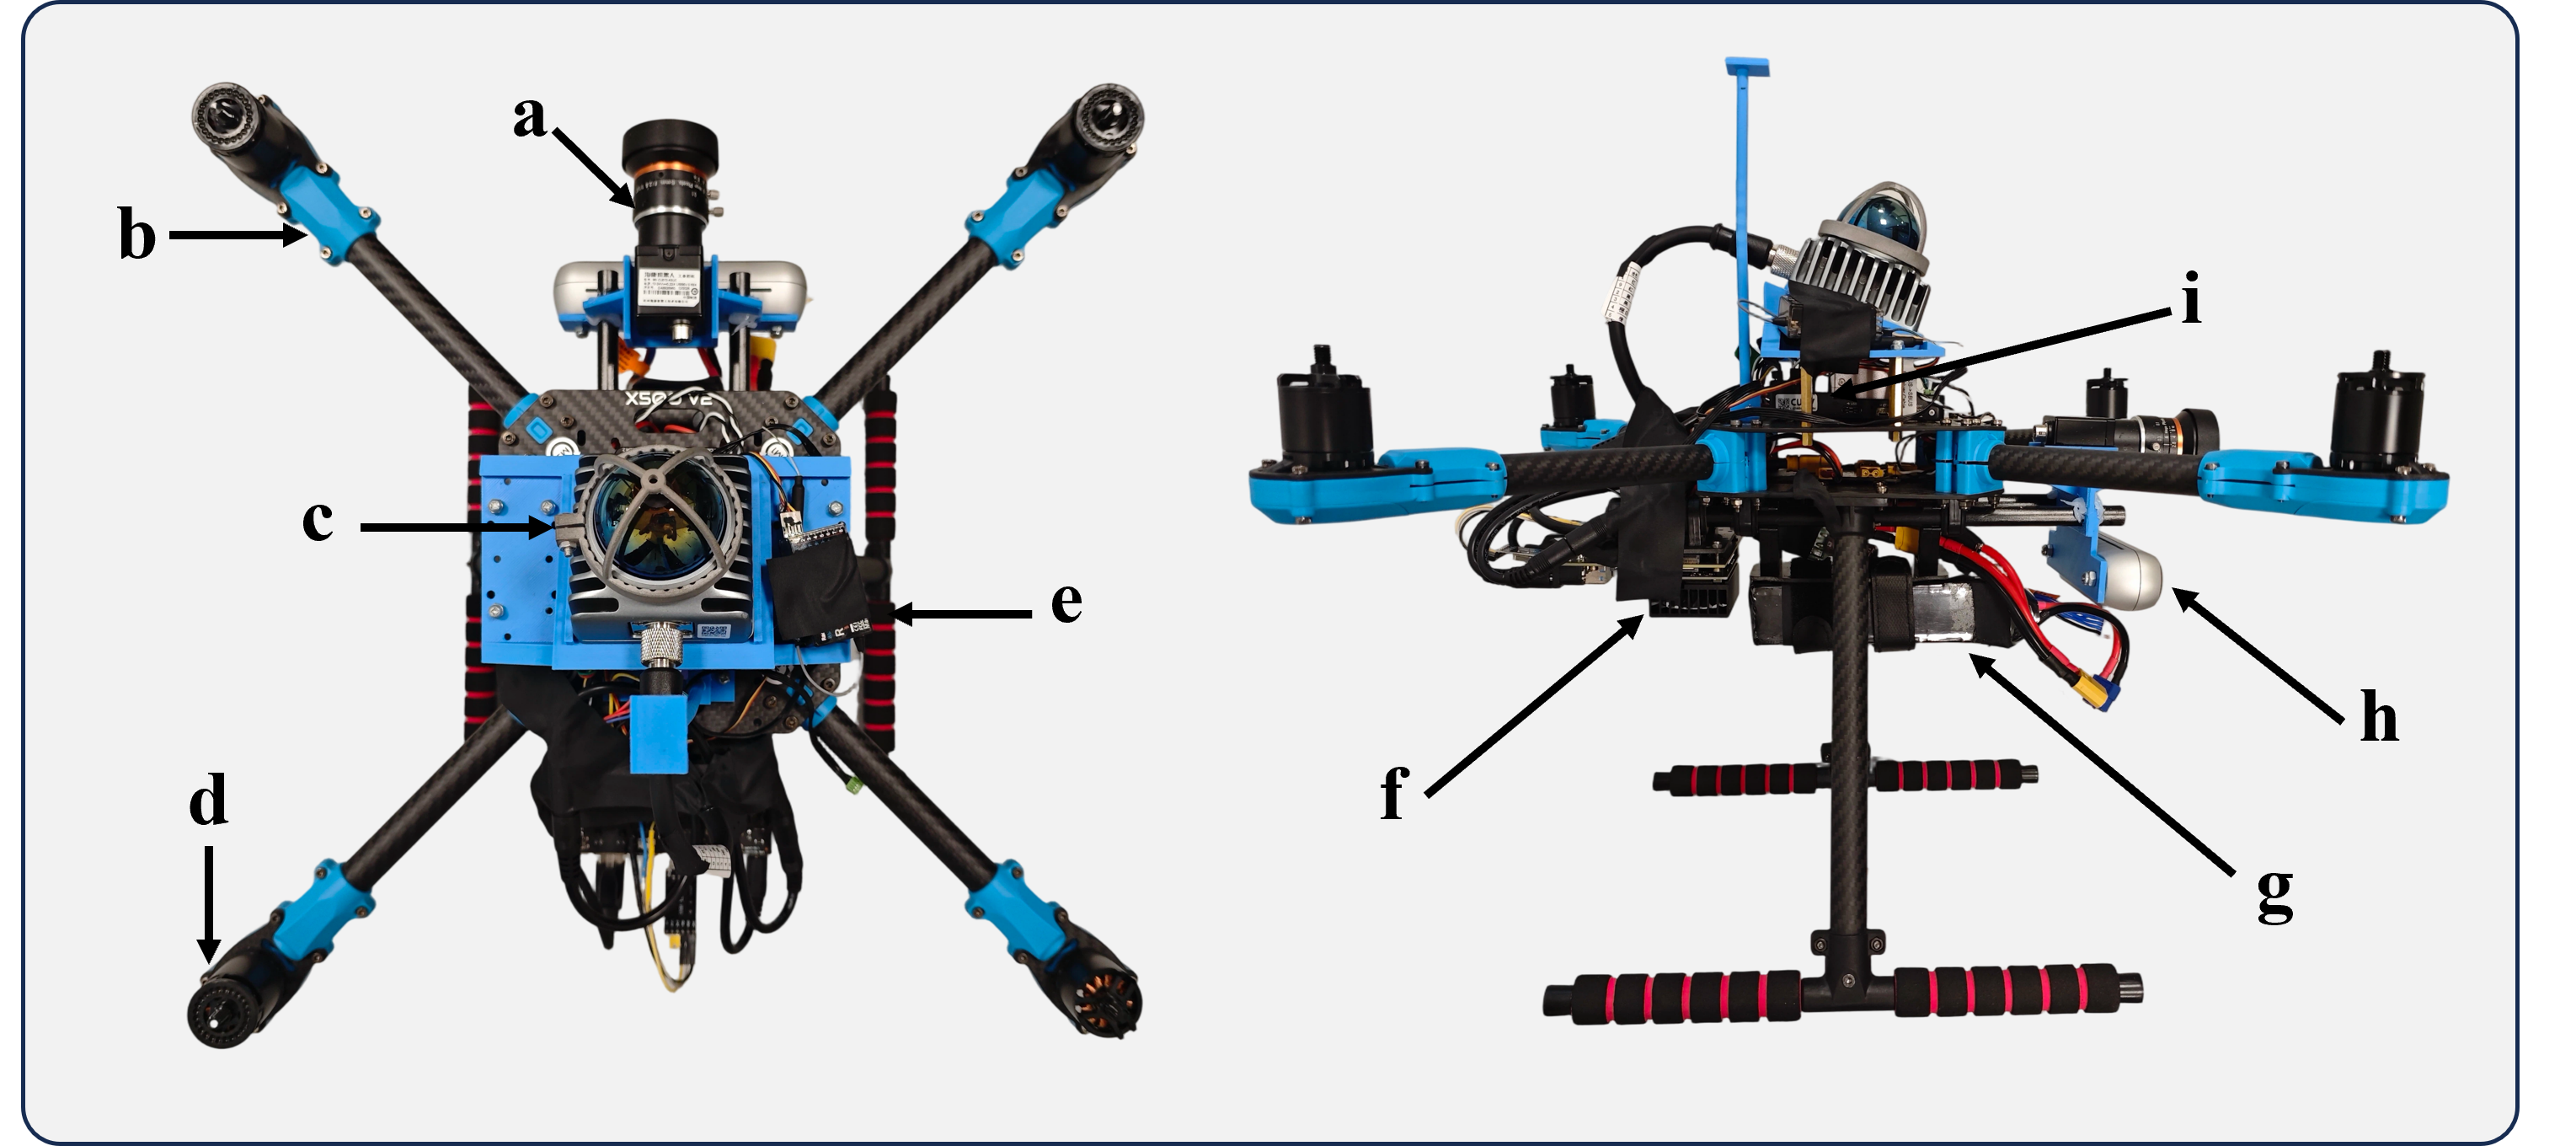
\includegraphics[width=0.9\textwidth]{figures/UAV}
    \caption{UAV platform and its main components:(a) LiDAR, 
    (b) frame, (c) monocular camera, (d) motor, (e) receiver, 
    (f) onboard computer, (g) power supply, 
    (h) stereo camera, and (i) flight controller.}
    \label{fig:UAV-platform}
\end{figure}

\subsection{Real-to-Sim Calibration}
The first design property is realized through a co-design between the real UAV
platform and the AirSim simulation environment. As stated above, real UAV
parameters constrain every scenario. Accordingly, the real platform defines the
engineering boundary of the rescue mission, while AirSim configures controllable
and repeatable scenarios within that boundary. Rather than treating the two as
separate experimental settings, we use the real platform to define the feasible
set from which AirSim configures each simulated UAV and its environment.
For each UAV, the configured mission must satisfy
\begin{equation}
\mathcal{E}_{\mathrm{UAV}}=
\left\{(h,v,m,e_{\mathrm{avail}},d)\;\middle|\;
\begin{aligned}
    h &\in \mathcal{H}_{\mathrm{safe}},\quad v \in \mathcal{V}_{\mathrm{safe}},\\
    m &\leq m_{\max},\quad e_{\mathrm{req}}+e_{\mathrm{res}} \leq e_{\mathrm{avail}},\\
    d &\leq d_{\mathrm{link}}
\end{aligned}
\right\},
\label{eq:uav-envelope}
\end{equation}
where $h$, $v$, $m$, $e_{\mathrm{avail}}$, and $d$ denote flight altitude,
velocity, payload mass, available energy, and distance to the coordination link. The safe altitude
and velocity ranges are specified by the operating policy. The payload and energy
bounds are grounded in the airframe, propulsion system, and battery; the energy
reserve enforces a safe return; and the link bound is determined by the deployed
communication configuration. Thus, the numerical bounds combine hardware
specifications, flight-safety policy, and deployment configuration. Any
configuration that violates
Eq.~\ref{eq:uav-envelope} is excluded before scenario generation. The real UAV
platform is shown in Figure~\ref{fig:UAV-platform}, and its hardware
specifications are listed in Table~\ref{tab:real_uav_hardware}.

% Required packages in the main document:
% \usepackage{booktabs}
% \usepackage{tabularx}
% \usepackage{array}

\begin{table*}[t]
    \centering
    \caption{Technical specifications of the real UAV platform.}
    \label{tab:real_uav_hardware}
    \small
    \setlength{\tabcolsep}{5pt}
    \renewcommand{\arraystretch}{1.15}

    \begin{tabularx}{\textwidth}{
        @{}
        >{\raggedright\arraybackslash}p{2.3cm}
        >{\raggedright\arraybackslash}p{3.2cm}
        >{\raggedright\arraybackslash}X
        @{}
    }
        \toprule
        \textbf{Subsystem} &
        \textbf{Model} &
        \textbf{Key specifications} \\
        \midrule

        UAV frame &
        Holybro X500 V2 &
        Carbon-fiber quadrotor frame, 500-mm wheelbase,
        approximately 610-g frame weight, and 1.5-kg published
        payload capacity excluding the battery at 70\% throttle. \\

        Flight controller &
        Holybro Pixhawk 6X &
        STM32H753 processor at 480 MHz, triple-redundant IMUs,
        dual barometers, 16 PWM outputs, two CAN buses,
        and 100-Mbps Ethernet. \\

        Companion computer &
        NVIDIA Jetson Orin NX 8 GB &
        6-core Arm Cortex-A78AE CPU, NVIDIA Ampere GPU,
        8-GB LPDDR5 memory, up to 117 TOPS,
        and configurable 10--40-W power modes. \\

        LiDAR &
        Livox Mid-360 &
        $360^{\circ}$ horizontal and $-7^{\circ}$--$52^{\circ}$
        vertical field of view, 200,000 points/s, 10-Hz frame rate,
        40-m range at 10\% reflectivity, 0.1-m blind zone,
        265-g weight, and 6.5-W average power. \\

        RGB-D camera &
        Intel RealSense D455 &
        Global-shutter stereo depth camera,
        $87^{\circ}\times58^{\circ}$ depth field of view,
        depth resolution up to $1280\times720$ at 90 fps,
        approximately 0.6--6-m effective range,
        integrated IMU, USB 3.1 interface, and 116-g weight. \\

        Propulsion system &
        $4\times$ Holybro 2216 KV920 &
        Four 920-KV brushless motors, four 20-A ESCs,
        and $10\times4.5$-in propellers, with a maximum
        manufacturer bench thrust of approximately
        1.33 kgf per motor at 16 V. \\

        Battery &
        Dualsky XP3300-6HED &
        6S lithium-polymer battery, 3300-mAh capacity,
        22.2-V nominal voltage, 25.2-V fully charged voltage,
        and approximately 73.3-Wh nominal energy. \\

        \bottomrule
    \end{tabularx}
\end{table*}


The virtual observation process is further fixed by the real camera geometry.
Under a nadir-view, locally planar-ground approximation, for altitude $h$,
horizontal field of view $\theta_{\mathrm{FOV}}$, and horizontal
resolution $N_x$, the image footprint and ground sampling distance are
\begin{equation}
W(h)=2h\tan\left(\frac{\theta_{\mathrm{FOV}}}{2}\right),\qquad
\mathrm{GSD}(h)=\frac{W(h)}{N_x}.
\label{eq:observation-geometry}
\end{equation}
Thus, the AirSim camera pose and the scale, density, and placement of fire-risk
elements are jointly constrained by what the real camera could observe, rather
than selected independently. Energy and payload limits likewise constrain route
length, task duration, and suppressible workload. Table~\ref{tab:real_to_sim_calibration}
records these calibration rules and the resulting simulation settings.

\begin{table*}[t]
    \centering
    \caption{Real-to-sim calibration of AirSim UAV and environment settings.}
    \label{tab:real_to_sim_calibration}
    \footnotesize
    \setlength{\tabcolsep}{5pt}
    \renewcommand{\arraystretch}{1.25}
    \begin{tabularx}{\textwidth}{
        @{}
        >{\raggedright\arraybackslash}p{2.7cm}
        >{\raggedright\arraybackslash}p{4.4cm}
        >{\raggedright\arraybackslash}X
        @{}
    }
        \toprule
        \textbf{Calibration target} &
        \textbf{Real-platform basis} &
        \textbf{AirSim configuration} \\
        \midrule
        Imaging geometry &
        Operating altitude and the RGB-D camera field of view and resolution &
        Observation height $h$, camera pose, field of view, and resolution; the resulting footprint $W(h)$ and GSD determine the observable ground area and image scale. \\

        Energy model &
        Battery capacity, propulsion characteristics, and return-to-base reserve policy &
        Available energy $e_{\mathrm{avail}}$, reserve $e_{\mathrm{res}}$, and energy consumption for flight and task execution. \\

        Payload model &
        Airframe and propulsion payload limit &
        Maximum payload $m_{\max}$ and the onboard suppressant inventory for each simulated UAV. \\

        Communication model &
        Deployed communication configuration and operating range &
        Link-distance threshold $d_{\mathrm{link}}$ and the distance-dependent connectivity condition. \\
        \bottomrule
    \end{tabularx}
\end{table*}


\subsection{Scenario Engineering}
The second design property is that each benchmark instance is purpose-built
rather than randomly sampled.
Each instance is generated from a controlled rescue configuration that specifies
the fire-risk layout, UAV states, mission constraints, and, when applicable, an
event schedule.

To make this construction systematic, each benchmark instance is represented
as a structured rescue state $S=\{O,F,R,U,C,E\}$, maintained by the generator.
Here, $O$ denotes aerial observations; $F$ fire-risk elements; $R$ risk regions;
$U$ UAV operational states; $C$ mission constraints; and $E$ event-driven
perturbations. Together, these elements define the rescue world but are not
exposed to the model as a single input.

The benchmark instead uses a stage-specific input--output format.
At mission start, the model receives $X_0=\{O,U,C\}$.
The fire-risk elements $F$ and risk regions $R$ are hidden annotations
that the model must infer from the observation. When a runtime event occurs,
the model receives the updated UAV state $U_t$ together with the event $E_t$.
The required outputs are the predicted $F$ and $R$, an initial mission plan $P$,
and, when applicable, a revised plan $P'$. Each instance carries hidden
ground-truth annotations for $F$ and $R$ to define fire-risk targets, risk
regions, and downstream task completion.
This standardized format makes the benchmark reusable
across different models and evaluation runs.

Finally, instances are assigned to one of the four progressive stress-testing
regimes summarized in Table~\ref{tab:scenario-controls}. At generation time,
the regime is specified by the initial condition $X_0$ and, when dynamic
conditions apply, a hidden event schedule $E$. Although $E$ is disclosed to the
model only upon occurrence, it is fixed in advance to control the closed-loop
difficulty of the instance. Each higher regime retains the requirements of lower
regimes while adding perception, resource, or dynamic coordination pressure.

\begin{table}[htbp]
    \centering
    \caption{Four difficulty levels and their controlled scenario conditions.}
    \label{tab:scenario-controls}
    \footnotesize
    \setlength{\tabcolsep}{4.5pt}
    \renewcommand{\arraystretch}{1.2}
    \begin{tabularx}{\textwidth}{
        @{}
        >{\raggedright\arraybackslash}p{1.5cm}
        >{\raggedright\arraybackslash}X
        >{\raggedright\arraybackslash}X
        >{\raggedright\arraybackslash}X
        @{}
    }
        \toprule
        \textbf{difficulty levels} &
        \textbf{Fire-point configuration} &
        \textbf{Fleet/resource conditions} &
        \textbf{Dynamic conditions} \\
        \midrule
        Simple &
        Sparse static fire points; few task zones. &
        Ample energy and payload. &
        None. \\

        Normal &
        Multiple fire points and task zones. &
        Multi-UAV allocation; normal resource margin. &
        None. \\

        Hard &
        Multi-region fire scene. &
        Energy or payload constrained. &
        Single perturbation. \\

        Expert &
        Dense or spreading fire-point layout. &
        Competing resource demands. &
        Concurrent perturbations; communication degradation. \\
        \bottomrule
    \end{tabularx}
\end{table}


\subsection{Evaluation Protocol}
The third design property is that the benchmark evaluates end-to-end model
behavior along an explicit decision chain and through multi-dimensional metrics,
rather than a single aggregated score. We formalize the decision chain as
\[
\begin{gathered}
O \rightarrow F \rightarrow R,\qquad (R,U,C) \rightarrow P, \\
(P,U_t,E_t) \rightarrow P'.
\end{gathered}
\]
Each relation represents one stage of the closed-loop rescue process.
$O \rightarrow F$ denotes fire-risk identification from aerial observations.
$F \rightarrow R$ denotes the abstraction of discrete fire elements
into coherent risk regions.
$R, U, C \rightarrow P$ denotes plan generation
from risk regions, UAV states, and mission constraints.
$P, U_t, E_t \rightarrow P'$ denotes plan revision from the current UAV
state under a runtime event.
Each step in this chain corresponds to the capabilities
provided by the system modules described in the System Overview.
Rather than scoring each intermediate representation independently, the protocol
evaluates whether the complete decision chain produces an effective executable
mission.

The protocol reports the six mission-level metrics in
Table~\ref{tab:evaluation-metrics}.

\begin{table}[htbp]
    \centering
    \caption{Mission-level evaluation metrics.}
    \label{tab:evaluation-metrics}
    \small
    \setlength{\tabcolsep}{5pt}
    \renewcommand{\arraystretch}{1.15}
    \begin{tabularx}{\textwidth}{
        @{}
        >{\raggedright\arraybackslash}p{3.0cm}
        >{\raggedright\arraybackslash}X
        @{}
    }
        \toprule
        \textbf{Metric} &
        \textbf{Evaluation focus} \\
        \midrule
        Completion &
        Successful handling of fire points or task zones by the fleet. \\

        Response &
        Timeliness of effective intervention after fire detection. \\

        Mission time &
        Efficiency in completing the full rescue mission. \\

        Event stability &
        Mission continuity under runtime perturbations and replanning. \\

        Resource pressure &
        Fleet-level and per-UAV resource consumption. \\

        Coordination &
        Balance of workload, flight distance, and execution duration across UAVs. \\
        \bottomrule
    \end{tabularx}
\end{table}


All applicable mission-level metrics are reported both overall and for each of
the four stress-testing regimes. Event stability is reported only for the Hard
and Expert regimes, where dynamic events occur. This regime-wise reporting
reveals whether a model fails under increasing perception, resource, or dynamic
coordination pressure.

Together, the structured scenario state and the evaluation protocol
define what the benchmark measures and how.
$S$ defines the rescue world the model must operate in, and the evaluation chain
defines the capabilities it must demonstrate. The mission-level metrics provide
a multi-dimensional profile of model behavior. Together with the structured
scenarios and standard formats, they support reproducible evaluation and
diagnostic comparison across models.

\endinput
